\subsection{Equilibrio de mercado parcial: un modelo no lineal}

Si el modelo de mercado aislado se sustituye por una función de demanda cuadrática, mientras que la función de oferta sigue siendo lineal, y se utilizaran coeficientes numéricos en vez de parámetros. Podria surgir un modelo como el siguiente
\begin{equation}
    \begin{aligned}
        Q_d &= Q_s \\
        Q_d &= 4-P^2 \\
        Q_s &= 4P-1
    \end{aligned}
\end{equation}
Este sistema de tres ecuaciones también se puede reducir a una sola ecuación mediante eliminación de variables 
\[
4-P^2 = P-1
\]
o bien 
\[P^2+4P -5 = 0\]
Si observa detenidamente, se encuentra frente a una ecuación cuadrática. A diferencia de la lineal, la ecuación cuadrática produce dos valores de solución.

\subsubsection{Ecuación cuadrática versus función cuadrática}

La expresión \(p^2+4P=5\) constituye una función cuadrática \(f(p)\), por lo tanto 
\[
f(p)= P^2+4P-5
\]
La función lo que hace es especificar una regla de asignación de \(P\) a \(f(p)\), como 
\begin{tabular}{|l|c|c|c|c|c|c|c|}
\hline
$P$    & $\dots$ & $-6$ & $-5$ & $-4$ & $-1$ & $0$  & $1$ \\ \hline
$f(P)$ & $\dots$ & $7$  & $0$  & $-5$ & $-8$ & $-5$ & $0$ \\ \hline
\end{tabular}

Aunque solo se listaron siete valores de \(P\) en esta tabla, en realidad todos los valores de \(P\) que se encuentren dentro del dominio de \(f(p)\) son elegibles para listar. Es por esto que rara vez se habla de ``resolver'' la ecuación \(f(p) = P^2 +4P - 5\), porque normalmente se espera que los valores de solución sean pocos, pero pueden intervenir todos los valores. Todo par ordenado de la tabla, se puede considerar un punto, se puede escribir una cantidad infinita de pares ordenados, lo cual indica que hay un número infinito de soluciones para \(f(p) = P^2 +4P - 5\).

Cuando se grafica \(f(p) = P^2 +4P - 5\), nos da como resultado la parábola de la figura \ref{Gráfica_cuadratica_modelo_no_lineal_1}

\begin{figure}[htbp]
    \centering
    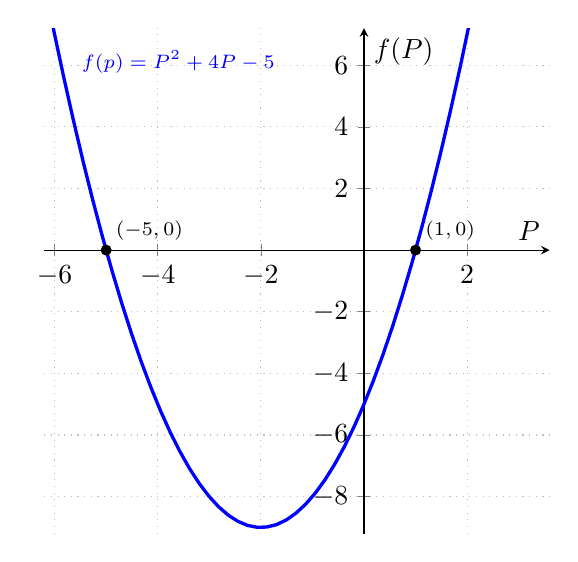
\begin{tikzpicture}
        \begin{axis}[
            axis lines = middle,
            xlabel = $\scriptsize{P}$,
            ylabel = $\scriptsize{f(P)}$,
            xmin=-6.2, xmax=3.6,
            ymin=-9.2, ymax=7.2,
            grid = major,
            major grid style= {dotted},
            width=8cm, height=8cm,
        ]

        % Ecuación: f(p) = P^2 +4P - 5
        \addplot [
            domain=-6.2:3, 
            samples=50, 
            color=blue, 
            very thick
        ] {x^2+4*x-5};

        % Etiquetas
        \node[color=blue] at (axis cs:-3.6, 6.1) {\scriptsize{$f(p)=P^2+4P-5$}};

        % Puntos
        \fill (1,0) circle (2 pt) node[above right] {\scriptsize{$(1,0)$}};
        \fill (-5,0) circle (2 pt) node[above right] {\scriptsize{$(-5,0)$}};

        \end{axis}
    \end{tikzpicture}
    \caption{\(f(p)=P^2+4P-5\)}
    \label{Gráfica_cuadratica_modelo_no_lineal_1}
\end{figure}

Cuando la función se iguala a \(0\), es decir \(P^2+4P -5 = 0\), la situación descripta anteriormente cambia de forma fundamental. Como desaparece la variable \(f(p)\) el resultado es una \textit{ecuación cuadrática} con la \textit{única} variable \(P^2\). Ahora \(f(p)\) esta restringida al valor cero, y solo una cantidad selecta de valores \(P\) (dos valores) pueden satisfacer y calificar como valores de solución. Como se ve en la figura de la parabola \ref{Gráfica_cuadratica_modelo_no_lineal_1}, los valores de solución, son aquellos que curzan el eje de \(x\), a estos valores se les denomina \textit{raíces} de la ecuación. Las raices son los puntos \((1,0)\) y \((-5,0)\). 

El valor de solución es el primer elemento de cada par de raiz, es decir, el valor de solución \(P\) es 
\[
P_1^\ast = 1 \qquad \qquad P_2^\ast = -5
\]
Como en económia se descartan los precios negativos, sólo es admisible el primer valor de solución.



\subsubsection{Fórmula cuadrática}

La ecuación \(P^2+4P -5 = 0\) fue resuelta de forma gráfica, pero tambien se puede resolver mediante un metodo algebraico. Dada la ecuación cuadratica de la forma 
\[
ax^2+bx+c=0 \qquad \qquad (a \neq 0)
\]
Se puede aplicar la \textit{fórmula cuadrática} para obtener las dos raices, esta es 
\[
x_1^\ast, x_2^\ast = \frac{-b \pm \sqrt{b^2-4ac}}{2a}
\]
donde el signo \(+\) produce \(x_1^\ast\) y el signo \(-\) produce \(x_2^\ast\).

Mientras que \(b^2-4ac>0\), van a diferir los valores de \(x_1^\ast\) y \(x_2^\ast\), lo que nosd a dos números reales como raíces. En el caso que \(b^2-4ac = 0\), \(x_1^\ast = x_2^\ast = -b/2a\), lo que significa que las raíces comparten el mismo valor, es decir son \textit{raíces repetidas}. Hay otro caso donde \(b^2-4ac<0\), lo cual nos obligaria a sacar la raíz cuadrada de un número negativo, lo cual no es posible en el sistema de números reales (esto se analizara más adelante).

Pero ¿Cómo conseguimos llegar a la \textit{fórmula cuadrática}? Esto se puede realizar por medio de un proceso conocido como ``completar al cuadrado''. Al dividir cada término de \(ax^2+bx+c=0\) entre \(a\) se obtiene la ecuación 
\[
\frac{ax^2}{a}+\frac{bx}{a}+\frac{c}{a}=0
\]
nos queda 
\[
x^2+\frac{bx}{a}+\frac{c}{a}=0
\]
Si restamos \(c/a\) y sumamos \(b^2/4a^2\) a ambos lados de la ecuación nos queda que 
\[
x^2+\frac{bx}{a}+\frac{c}{a} + \frac{b^2}{4a^2} - \frac{c}{a} = + \frac{b^2}{4a^2} - \frac{c}{a}
\]
Realizando las operaciones que tenemos nos queda de forma simplificada que 
\[
x^2+\frac{b}{a}x + (\frac{b}{4a})^2 = + \frac{b^2}{4a^2} - \frac{c}{a}
\]
El lado izquierdo ahora es un ``cuadrado perfecto'' \(((m+n)^2=m^2+2mn+n^2)\), donde el primer y tercer término coincide con la ecuación que tenemos arriba, en el caso del segundo término, si lo calculamos tomando \(m = x\) y \(n=b/2a\), nos queda que \(2(x)(b/2a)\), se cancela el \(2\) y nos queda \(x(b/a)\), es decir el segundo término. Por lo tanto, la ecuación se puede expresar como 
\[
(x+\frac{b}{2a})^2 = + \frac{b^2}{4a^2} - \frac{c}{a}
\]
En el caso de la parte derecha de la ecuación, debemos realizar una resta de fracciones. Como para restar una fracción necesitamos un denominador común, en este caso \(4a^2\), la primera fracción ya lo tiene, pero la segunda no. Como a \(c/a\) le falta \(4a\) para llegar a \(4a^2\), le multiplicamos \(4a\) arriba como abajo, quedandonos \(c4a/4a^2\). Como ahora los denominadores son iguales, restamos, resultando
\[
(x+\frac{b}{2a})^2 = \frac{b^2-4ac}{4a^2}
\]
Sí ahora sacamos la raíz cuadrada en ambos lados, nos queda que  (recordar que \(\sqrt{a/b} = \sqrt{a}/\sqrt{b}\))
\[
x+\frac{b}{2a} = \pm \frac{\sqrt{b^2-4ac}}{2a}
\]
Por ultimo si de ambos lados restamos \(b/2a\), obtenemos
\[
x = -\frac{b}{2a} \pm \frac{\sqrt{b^2-4ac}}{2a}
\]
Realizamos una resta de fracciones, dando la \textit{fórmula cuadrática}
\[
x_1^\ast, x_2^\ast = \frac{-b \pm \sqrt{b^2-4ac}}{2a}
\]

Si remplazamos la formula paramétrica con los datos de nuestro ejercicio, nos queda que 
\[
P_1^\ast, P_2^\ast = \frac{-4 \pm \sqrt{4^2-4(1\times-5)}}{2\times1} = \frac{-4 \pm \sqrt{16+20}}{2} = \frac{-4 \pm 6}{2} = 1, -5
\]

Con esta información, la cantidad de equilibrio \(Q^\ast\) se obtiene a partir de remplazar, la ecuación \(Q_d = 4-P^2\) o \(Q_s = 4P-1\), remplazando \(P\), dando como resultado \(Q^\ast = 3\).



\subsubsection{Otra solución gráfica}

La figura \ref{Gráfica_cuadratica_modelo_no_lineal_1} presenta un método de solución gráfica del presente modelo. Sin embargo, como la cantidad variable se eliminó al deducir la ecuación cuadrática, solo se puede encontrar \(p^\ast\) en esa figura.

Si queremos determinar tanto \(P^\ast\) como \(Q^\ast\) de la grafica, se debe usar un diagrama con \(Q\) en un eje y \(P\) en el otro.

\begin{figure}[htbp]
    \centering
    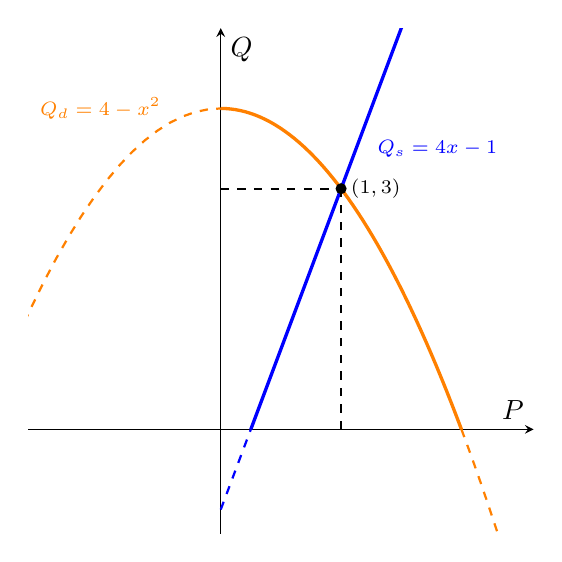
\begin{tikzpicture}
        \begin{axis}[
            axis lines = middle,
            xlabel = $P$,
            ylabel = $Q$,
            xmin=-1.6, xmax=2.6,
            ymin=-1.3, ymax=5,
            grid = major,
            major grid style= {dotted},
            width=8cm, height=8cm,
            ytick = \empty, xtick = \empty,
        ]
        
        % 1. TRAMO PUNTEADO
        \addplot [
            domain=0:0.25, 
            samples=2, 
            color=blue, 
            thick, 
            dashed
        ] {x*4-1};

        % 2. TRAMO SÓLIDO
        \addplot [
            domain=0.25:5, 
            samples=2, 
            color=blue, 
            very thick
        ] {4*x-1};


        % 3. TRAMO PUNTEADO
        \addplot [
            domain=-2:0, 
            samples=20, 
            color=orange, 
            thick, 
            dashed
        ] {4-x^2};

        % 4. TRAMO SÓLIDO
        \addplot [
            domain=0:2,
            samples=50,
            color=orange,
            very thick,
        ] {4-x^2};

        % 5. TRAMO PUNTEADO
        \addplot [
            domain=2:3, 
            samples=20, 
            color=orange, 
            thick, 
            dashed
        ] {4-x^2};

        % Etiquetas
        \node[color=blue] at (axis cs:1.8, 3.5) {\scriptsize{$Q_s = 4x-1$}};
        \node[color=orange] at (axis cs:-1, 4) {\scriptsize{$Q_d = 4-x^2$}};

        % --- PUNTO DE EQUILIBRIO Y PROYECCIONES ---
        % Definimos las coordenadas del equilibrio (P=2.7, Q=1.7)
        \coordinate (E) at (axis cs:1, 3);
            
        % Línea punteada hacia el eje Y (Cantidad)
        \draw [dashed, thick] (axis cs:0, 3) -- (E) node[left, pos=0.03] {};
            
        % Línea punteada hacia el eje X (Precio)
        \draw [dashed, thick] (axis cs:1, 0) -- (E) node[below, pos=0] {};
            
        % El punto físico del equilibrio
        \fill[black] (E) circle (2pt) node[right] {\scriptsize{$(1,3)$}};

        \end{axis}
    \end{tikzpicture}
    \caption{Determinación de la cantidad con la gráfica.}
    \label{Gráfica_cuadratica_modelo_no_lineal_2}
\end{figure}

El problema es encontrar la intersección de dos conjuntos de puntos, 
\begin{equation}
    \begin{aligned}
    D (\text{demanda}) &= \{(P,Q) | Q = 4 - P^2\} \\
    S (\text{oferta}) &= \{(P,Q) | Q = 4P - 1\} \\
    \end{aligned}
\end{equation} 
Si no se pone restricción en el dominio y la imagen, el conjunto de intersección contendrá dos elementos, a saber 
\[
D \cap S = \{((1,3),(-5,-21))\}
\]
Esto se puede observar en la gráfica \ref{Gráfica_cuadratica_modelo_no_lineal_2}. El primer punto se localiza en el primer cuadrante y el ultimo en el tercer cuadrante. So el dominio y la imagen se restringen a valores positivos, solo se puede aceptar el primer par ordenado, por lo tanto el equilibrio es único.


\subsubsection{Ecuaciones polinomiales de grado superior}

Si un sistema de ecuaciones simultáneas no se reducen a una ecuación lineal o a una ecuación cuadrática, sino a una cúbica o a una superior, será más difícil encontrar las raíces. Un método útil que puede funcionar es el de \textit{factorizar} la función.

\begin{ejemplo}
    \label{ejemplo_factorización}
    La expresión \(x^3-x^2-4x+4\) se puede escribir como el producto de tres factores \((x-1)\), \((x+2)\) y \((x-2)\), vea el procedimiento
    \[
    x^3-x^2-4x+4 = 0
    \]
    Realizamos la factorización por agrupación, donde dividimos en dos parejas y vemos que tienen en común 
    \[
    x^2(x-1)-4(x-1)=0
    \]
    Como nos quedo que se repite \((x-1)\), podemos volver a agrupar, quedandonos
    \[
    (x^2-4)(x-1)=0
    \]
    Por ultimo el término \((x^2-4)\) es una diferencia de cuadrados. La regla dice que \(a^2-b^2 = (a-b)(a+b)\), como \(4=2^2\) aplicamos diferencia de cuadrados
    \[
    (x-1)(x-2)(x+2)=0
    \]
    Como el producto del lado izquierdo debe ser \(0\), si cumplimos con la condición de igualdad, nos queda que 
    \begin{equation}
        \begin{aligned}
            x-1 = 0 \quad &\text{   Por lo tanto    } \quad x_1^\ast = 1 \\
            x+2 = 0 \quad &\text{   Por lo tanto    } \quad x_2^\ast = -2 \\
            x-2 = 0 \quad &\text{   Por lo tanto    } \quad x_3^\ast = 2 
        \end{aligned}
    \end{equation} 
\end{ejemplo}

En el ejemplo \ref{ejemplo_factorización} se ilustra dos hechos interesantes sobre la factorización. Primero, dada una ecuación polinomial de tercer grado, la factorización da como resultado tres términos de la forma \((x-raiz)\), y de este modo se obtienen tres raices. Por lo común, una ecuación polinomial de grado \(n\) debe producir un total de \(n\) raíces. Segundo, hay una relación entre las tres raíces \((1,-2,2)\) y el termino constante \((4)\). Como el término constante debe ser el producto de las tres raíces, cada raíz debe ser un \textit{divisor} del término constante. Esto se formaliza en el siguiente teorema

\paragraph{Teorema I}

Dada la ecuación polinomial
\[
x^n+a_{n-1}x^{n-1}+\dots+a_1x+a_0 = 0
\]
donde los coeficientes son enteros y el coeficiente \(x^n\) es la unidad, si existen raíces enteras, entonces cada una de ellas debe ser un divisor de \(a_0\).

Si el primer término \(x_n\) no tiene ningún número al lado (es decir, el coeficiente es \(1\)), las posibles soluciones enteras están ``escondidas'' dentro del último número \(a_0\). Si buscamos una solución hay que buscarlo en los divisores de \(a_0\).

Cuando se encuentran fracciones como coeficientes de la ecuación polinomia, como en 
\[
x^4+\frac{5}{2}x^3-\frac{11}{2}x^2-10x+6 = 0
\]
Estas no forman parte de la hipótesis del teorema I. Aun cuando se multiplique por \(2\) para eliminar las fracciones, no se puede aplicar el teorema I, porque el coeficiente de mayor grado no es la unidad. Lo que nos lleva al 

\paragraph{Teorema II}

Dada la ecuación polinomial con coeficientes enteros 
\[
a_nx^n + a_{n-1}x^{n-1}+\dots+a_1x+a_0 = 0
\]
si existe una raíz racional \(r/s\), donde \(r\) y \(s\) son enteros sin un divisor en común diferente de la unidad, entonces \(r\) es un divisor de \(a_0\) y \(s\) un divisor de \(a_n\).

En otras palabras, si el primer termino \(x_n\) no es \(1\), la solución puede ser una fraccion de \(r/s\), donde \(r\) es un divisor de \(a_0\) y \(s\) es un divisor del primer término \(a_n\).

\begin{ejemplo}
    \label{ejemplo_factorización_teorema_2}
    ¿Tiene la ecuación cuádratica \(2x^4+5x^3-11x^2-20x+12=0\) raíces racionales?

    Con \(a_0=12\), los unicos valores posible para el numerador \(r\) en \(r/s\) son el conjunto de divisores \(\{1,-1,2,-2,3,-3,4,-4,6,-6,12,-12\}\). Y con \(a_n=2\), los únicos valores posibles para \(s\) son el conjunto de divisores \(\{1,-1,2,-2\}\). 

    Si tomamos cada elemento del conjunto \(r\) y lo dividimos por cada elemento del conjunto \(s\), obtenemos que \(r/s\), sólo puede tomar los valores
    \[
    \pm 1, \pm \frac{1}{2}, \pm 2, \pm 3, \pm \frac{3}{2}, \pm 4, \pm 6, \pm 12
    \]
    Entre estos candidatos, muchos no satisfacen la ecuación dada. Por ejemplo, al remplazar \(x = 1\) en la ecuación cuártica se obtiene el resultado absurdo de \(-12 = 0\). Como se esta resolviendo una ecuación cuártica, se puede esperar a lo sumo cuatro de los valores \(r/s\) listados califiquen como raíces. Estos valores son en este caso \(1/2,2,-2,-3\). Según el principio de factorización, la ecuación cuartica dada se puede escribir en forma equivalente como 
    \[
    (x-\frac{1}{2})(x-2)(x+2)(x+3)=0
    \]
    donde el primer factor tamién se puede escribir como \(2x-1\).
\end{ejemplo}

En el ejemplo \ref{ejemplo_factorización_teorema_2} se rechaza la raiz posible \(1\) porque \(x=1\) no satisface la ecuación. Es decir, si sustituimos \(x\) por \(1\) en la ecuación, está no da la identidad de \(0=0\) como se requiere.
Pero si \(x=1\) es una raíz de alguna ecuación polinomial. En ese caso puesto que \(x^n=x^{n-1}=\dots=x=1\), la ecuación polinomial se reduciria a la forma simple \(a_n^n + a_{n-1}+\dots+a_1+a_0 = 0\). Este hecho proporciona el fundamento para el siguiente 

\paragraph{Teorema III}

Dada la ecuación polinomial 
\[
a_nx^n + a_{n-1}x^{n-1}+\dots+a_1x+a_0 = 0
\]
Si la suma de los coeficientes \(a_n,a_{n-1},\dots,a_0\) es cero, entonces \(x=1\) es una raíz de la ecuación.


\begin{ejercicio}
    \begin{enumerate}
        \item Determine los ceros de las siguientes funciones
        \[
        (a)\quad f(x)=x^2-8x+15 \qquad \qquad (b) \quad g(x) = 2x^2-4x-16
        \]
        \item \((a)\) Encuentre una ecuación cúbica con raíces \(6,-1\) y \(3\).
        
        \((b)\) Obtenga una ecuación cuártica con raíces \(1,2,3\) y \(5\).
        \item Para cada una de las siguientes ecuaciones polinomiales, determine si \(x=1\) es una raíz.
            \begin{equation}
                \begin{aligned}
                    &(a) \quad x^3-2x^2+3x-2=0 \qquad \qquad (b) \quad 2x^3 - \frac{1}{2}x^2+x-2=0 \\
                    &(c) \quad 3x^4-x^2+2x-4=0
                \end{aligned}
            \end{equation} 
        \item Halle las raíces racionales, si existen, de las siguientes ecuaciones.
            \begin{equation}
                \begin{aligned}
                    &(a) \quad x^3-4x^2+x+6=0 \qquad \qquad &&(b) \quad 8x^3 - 6x^2-3x-1=0 \\
                    &(c) \quad x^3+\frac{3}{4}x^2-\frac{3}{8}x-\frac{1}{8}=0  &&(d) \quad x^4 - 6x^3 + 7\frac{3}{4}x^2-\frac{3}{2}x-2=0
                \end{aligned}
            \end{equation}         
        \item Obtenga la solución de equilibrio para cada uno de los siguientes modelos
            \begin{equation}
                \begin{aligned}
                    (a)\quad & Q_d = Q_s  \qquad \qquad (b) \quad &&Q_d = Q_s \\
                    & Q_d=3-P^2    &&Q_d = 8-P^2 \\
                    & Q_s=6P-4     &&Q_s = P^2-2
                \end{aligned}
            \end{equation}         
        \item La condición de equilibrio de mercado, \(Q_d = Q_s\), suele expresarse en una forma alternativa equivalente, \(Q_d - Q_s = 0\), que tiene la interpretación económica ``la demanda excedente es cero''. ¿Representa la ecuación \(P^2+4P -5 = 0\) esta última versión de la condición de equilibrio? Si no, provea una interpretación apropiada para \(P^2+4P -5 = 0\)
    \end{enumerate}
    \emph{Respuestas}
    \begin{enumerate}
        \item \((a)\) \(x_1^*=5\) \(x_2^*=3\), \((b)\) \(x_1^*=4\), \(x_2^*=-2\)
        \item \((a)\) \(x^3-8x^2+9x+18\), \((b)\) \(x^4-11x^3+41x^2-61x+30\). El procedimiento es como el ejemplo \ref{ejemplo_factorización} pero a la inversa.
        \item \((a)\) Despues de aplicar el teorema I y resolver, encontramos que la raíz es \(1\). \((b)\) Es un numero irracional, por lo tanto no se encuentra una raiz racional. \((c)\) Aplicando el teorema II y resolviendo, nos da que la raíz es \(1\).
        \item \((a)\) Por teorema I, la raíz es \(3\) y \(2\). \((b)\) El número no es racional, no se puede resolver con teoremas. \((c)\) Por teorema I la raíz se encuentra en \(-1\). \((d)\) Las raices son irracionales.
        \item \((a)\) \(P^*=1\) y \(Q^*=2\) 
        
        \((b)\) \(P^*=\sqrt{5}\) y \(Q^*=3\)
        \item Cuando nos referimos a que la demanda excedente es cero, decimos que no se ofrecen productos de más, ni se demandan más productos. Es el punto donde ambas partes se benefician. La ecuación \(P2+4P-5=0\) representa la función de exceso de demanda \(E\) para un mercado específico. El valor de P que sea la raíz de esta ecuación será el precio que garantiza que el exceso de demanda sea nulo
    \end{enumerate}
\end{ejercicio}

